	%% ++++++++++++++++++++++++++++++++++++++++++++++++++++++++++++
%% Hauptdatei, Wurzel des Dokuments
%% ++++++++++++++++++++++++++++++++++++++++++++++++++++++++++++

% Headerfeld, Typ des Dokumentes, einzubindende Packages.
% Hier bei Bedarf Änderungen vornehmen.
\documentclass
[   twoside=false,     % Einseitiger oder zweiseitiger Druck?
    fontsize=12pt,     % Bezug: 12-Punkt Schriftgröße
    DIV=15,            % Randaufteilung, siehe Dokumentation "KOMA"-Script
    BCOR=17mm,         % Bindekorrektur: Innen 17mm Platz lassen. Copyshop-getestet.
%    headsepline,
    headsepline,  % Unter Kopfzeile Trennlinie (aus: headnosepline)
    footsepline,  % Über Fußzeile Trennlinie (aus: footnosepline)
    open=right,        % Neue Kapitel im zweiseitigen Druck rechts beginnen lassen
    paper=a4,          % Seitenformat A4
    abstract=true,     % Abstract einbinden
    listof=totoc,      % Div. Verzeichnisse ins Inhaltsverzeichnis aufnehmen
    bibliography=totoc,% Literaturverzeichnis ins Inhaltsverzeichnis aufnehmen
    titlepage,         % Titelseite aktivieren
    headinclude=true,  % Seiten-Head in die Satzspiegelberechnung mit einbeziehen
    footinclude=false, % Seiten-Foot nicht in die Satzspiegelberechnung mit einbeziehen
    numbers=noenddot   % Gliederungsnummern ohne abschließenden Punkt darstellen
]   {scrreprt}         % Dokumentenstil: "Report" aus dem KOMA-Skript-Paket

\usepackage[active]{srcltx}
\overfullrule=2cm
%\usepackage[activate=normal]{pdfcprot} % Optischer Randausgleich -> pdflatex!
\usepackage{ifthen}
\usepackage[ngerman]{babel}   % Neue Deutsche Rechtschreibung
%\usepackage[latin1]{inputenc} % Zeichencodierung nach ISO-8859-1
\usepackage[utf8]{inputenc}   %	Zeichencodierung nach UTF-8 (Unicode)
\usepackage[T1]{fontenc}
\usepackage{graphicx}
%\usepackage{ae} % obsolet und durch lmodern ersetzt
\usepackage{lmodern}
\usepackage{listings}
\usepackage[T1]{url}
\usepackage{amsthm}
\usepackage{amsmath}
\usepackage{graphicx}
\RequirePackage{scrlfile}
\ReplacePackage{scrpage2}{scrlayer-scrpage}
% old: \usepackage[automark]{scrpage2}
\usepackage[automark]{scrlayer-scrpage}
\usepackage{setspace}
%\usepackage[first,light]{draftcopy} % Für Probedruck
\usepackage[plainpages=false,pdfpagelabels,hypertexnames=false]{hyperref}

% Tiefe der Kapitelnummerierung beeinflussen
\setcounter{secnumdepth}{3} % Tiefe der Nummerierung
\setcounter{tocdepth}{3}    % Tiefe des Inhaltsverzeichnisses

% Datum anpassen
\newcommand{\leadingzero}[1]{\ifnum #1<10 0\the#1\else\the#1\fi}
\renewcommand{\today}{\leadingzero{\day}.\leadingzero{\month}.\the\year}     % DD.MM.YYYY

% Hier in die zweite geschweifte Klammer jeweils
% die persoenlichen Daten und das Thema der Arbeit eintragen:
\newcommand{\artderausarbeitung}{Pflichtenheft}
\newcommand{\namedesautors}{P.~Augustin, C.~Juin, G.~Lehmann, A.~Schmidt, R.~Schöne}
\newcommand{\themaderarbeit}{RION  Package-Manager}
\newcommand{\xRION}{\RION}

% PDF Metadaten definieren
\hypersetup{
   pdftitle={\themaderarbeit},
   pdfsubject={\artderausarbeitung},
   pdfauthor={\namedesautors},
   pdfkeywords={\artderausarbeitung; TU-Ilmenau}}


% Abkürzungsverzeichnis beeinflussen. Hier nichts ändern!
\usepackage[intoc]{nomencl}
  \AtBeginDocument{\setlength{\nomlabelwidth}{.25\columnwidth}}
  \let\abbrev\nomenclature
  \renewcommand{\nomname}{Abkürzungsverzeichnis und Formelzeichen}
  \renewcommand{\nomlabel}[1]{#1 \dotfill}
  \setlength{\nomitemsep}{-\parsep}
  \makenomenclature

\usepackage[normalem]{ulem}
  \newcommand{\markup}[1]{\textbf{#1}}

% Seitenlayout festlegen. Hier nichts ändern!
\pagestyle{scrplain}
\ihead[]{\headmark}
\ohead[]{\pagemark}
\chead[]{}
\ifoot[]{}
\ofoot[]{\scriptsize \artderausarbeitung\ \namedesautors}
\cfoot[]{}
\renewcommand{\titlepagestyle}{scrheadings}
\renewcommand{\partpagestyle}{scrheadings}
\renewcommand{\chapterpagestyle}{scrheadings}
\renewcommand{\indexpagestyle}{scrheadings}



% Abschnittsweise Nummerierung anstatt fortlaufend. Hier nichts ändern!
\makeatletter
\@addtoreset{equation}{chapter}
\@addtoreset{figure}{chapter}
\@addtoreset{table}{chapter}
\renewcommand\theequation{\thechapter.\@arabic\c@equation}
\renewcommand\thefigure{\thechapter.\@arabic\c@figure}
\renewcommand\thetable{\thechapter.\@arabic\c@table}
\makeatother
\renewcommand*{\pagedeclaration}[1]{\unskip, \hyperpage{#1}}

% Quelltextrahmen, klein. Hier nichts ändern!
\newsavebox{\inhaltkl}
\def\rahmenkl{\sbox{\inhaltkl}\bgroup\small\renewcommand{\baselinestretch}{1}\vbox\bgroup\hsize\textwidth}
\def\endrahmenkl{\par\vskip-\lastskip\egroup\egroup\fboxsep3mm%
\framebox[\textwidth][l]{\usebox{\inhaltkl}}}

% Quelltextrahmen, normale Groesse. Hier nichts ändern!
\newsavebox{\inhalt}
\def\rahmen{\sbox{\inhalt}\bgroup\renewcommand{\baselinestretch}{1}\vbox\bgroup\hsize\textwidth}
\def\endrahmen{\par\vskip-\lastskip\egroup\egroup\fboxsep3mm%
\framebox[\textwidth][l]{\usebox{\inhalt}}}


% Sonstige Befehlsdefinitionen hier ablegen.
\newcommand{\entspricht}{\stackrel{\wedge}{=}}
\newcommand{\quotes}[1]{\glqq#1\grqq{}}
\newcommand{\x}{X-FAB} % sry :)
\newcommand{\e}{RION} % well
\newcommand{\Linux}{GNU/Linux}
\makenomenclature


% Tabellenspaltendefinitionen mit fester Breite --> somit Zeilenumbruch innerhalb einer Zelle möglich
% aus http://www.torsten-schuetze.de/tex/tabsatz-2004.pdf
\usepackage{array, booktabs}
\newcolumntype{f}{>{$}l<{$}}
\newcolumntype{n}{>{\raggedright}l}
\newcolumntype{N}{>{\scriptsize}l}
\newcolumntype{v}[1]{>{\raggedright\hspace{0pt}}m{#1}}
\newcolumntype{V}[1]{>{\scriptsize\raggedright\hspace{0pt}}m{#1}}
\newcolumntype{Z}[1]{>{\raggedright\centering}m{#1}}
\newcolumntype{k}[1]{>{\raggedright}p{#1}}
% ergibt Tabllenspalte fester Breite, linksbündig
% Umbruch innerhalb der Zelle mit \\, neue Tabellezeile mit \tabularnewline
% \addlinespace für Gruppentrennung (aus \texttt{booktabs.sty})


\begin{document}
\onehalfspacing

\begin{titlepage}
	\centering
	{\Large \textsc{Technische Universität Ilmenau}}\\[3ex]
	{\Large Rechnerarchitekturen und Eingebettete Systeme}\\[3ex]
	\vfill
	{\Large \textbf{\artderausarbeitung}}\\[4ex]
	{\large \textbf{\themaderarbeit}}\\[5ex]
	%{\large \textbf{\xRION}}\\[5ex]
	\vfill
	\begin{tabular}{rl}
		\hline\\
		vorgelegt von:          & \quad \namedesautorsI\\[1,5ex]
										       & \quad \namedesautorsII\\[1,5ex]
		eingereicht am:         & \quad 
		\today \\[1,5ex]
		Fachgebiet:            & \quad Rechnerarchitekturen und Eingebettete Systeme\\[0,5ex]
								& \quad Institut für Mikroelektronik- und Mechatronik-System\\[1,5ex]
		Betreuer:            	& \quad Georg Gläser, Andreas Becher \\[1,5ex]
		Seminarleiter           & \quad Prof. Armin Zimmermann \\[1,5ex]	
	\end{tabular}
	\vfill
	
    


\end{titlepage}
%%% ++++++++++++++++++++++++++++++++++++++++++++++++++++++++++++
%% Zusammenfassung, Abstract
%% ++++++++++++++++++++++++++++++++++++++++++++++++++++++++++++


\renewcommand{\abstractname}{Kurzfassung}
\begin{abstract}
	\begin{center}
		X-FAB bietet eine Fülle an unterschiedlichen Technologien für diverse und auch
        spezifische Anwendungsmärkte an. Um Packete für das Process Design Kit verwalten zu können soll ein Package-Manager mit dem Namen RION geschaffen werden
	\end{center}
\end{abstract}

% Inhaltsverzeichnis
\cleardoublepage % Seitenumbruch erzwingen vor Änderung des Nummerierungsstils
\pagenumbering{roman} % Nummerierung der Seiten ab hier: i, ii, iii, iv...
\pagestyle{scrheadings} % Ab hier mit Kopf- und Fusszeile
\tableofcontents

% Die einzelnen Kapitel
\cleardoublepage % Seitenumbruch erzwingen vor Änderung des Nummerierungsstils
\pagenumbering{arabic} % Nummerierung der Seiten ab hier: 1, 2, 3, 4...

%%% Content %%%
\part*{Pflichtenheft}

%% Pages
\chapter{Zielbestimmungen}

Rion ist ein Package-Manager zum Suchen, Installieren, Aktualisieren und verwalten von Packages für das PDK. Die Pakete für Rion werden von der Serverseite Endor verwaltet.

\section{Problemstellung}
Zur Zeit werden Packages manuell von einem Webinterface heruntergeladen. Sie werden manuell installiert und manuell aktualisiert. Dieser jetzige Weg ist jedoch unübersichtlich, kostet sehr viel Zeit und erfordert sehr viel manuelle Arbeit. Daher soll dieser Prozess durch Verwendung von Rion vereinfacht und automatisiert werden.

\section{Musskriterien}
\subsection{Funktionalität}
\begin{itemize}
		\item Endor muss die Packages serverseitig über eine Datenbank in Form von Archiven zur Verfügung stellen.
		\item Rion muss eine Liste der auf dem Server vorliegenden Pakete herunterladen und durchsuchen können.
		\item Rion muss Pakete instalblieren können. Dabei müssen auch ältere Versionen des Paketes zugänglich gemacht werden können.
		\item Rion muss installierte Pakete aktualisieren können. In diesem Kontext bedeutet, dies die neuere Version des Paketes parallel zur Alten zu installieren.
		\item Rion muss installierte Pakete entfernen können.
\end{itemize}

\subsection{Interaktion}


\begin{itemize}
	\item Dem Benutzer muss ein CLI zur Verfügung stehen.
\end{itemize}

\section{Wunschkriterien}
\begin{itemize}
	\item Endor soll Pakete signieren.
	\item Endor soll Hashwerte von Paketen anfertigen und an Rion übermitteln können.
	\item Rion soll nach dem Herunterladen, aber vor der Installation, Pakete auf ihre Signatur, sowie auf ihren korrekten Hashwert überprüfen.

\end{itemize}
\chapter{Vorgehensmodell}
\section{Motivation und Auswahl des Vorgehensmodells}

Als Vorgehensmodell haben wir uns aufgrund der interdisziplinären Zusammensetzung und Größe unseres Teams, sowie der Forderung nach einem agilen Vorgehensmodell seitens der X-FAB für Scrum entschieden.\\
Weiterhin ermöglicht es Scrum durch iteratives Vorgehen flexibel auf Anforderungsänderungen zu reagieren und in jeder Iteration einen funktionsfähigen Prototyp fertigzustellen.\\

Scrum benötigt folgende Rollen innerhalb des Teams:
\begin{itemize}
	\item[Product Owner:] Durch ihn erfolgt eine kontinuierliche Qualitätssicherung der Prototypen. Des Weiteren führt er den Product-Backlog und dokumentiert somit den Gesamtfortschritt des Projekts.

	\item[Scrum Master:] Er moderiert interne Meetings, achtet auf die Einhaltung der Scrum-Methoden, hilft bei der Formulierung der Zielstellungen und unterstützt alle Mitglieder bei aufkommenden Problemen innerhalb ihrer Aufgaben.
	
	\item[Developer:]
	Sind für die Umsetzung der Sprint-Ziele verantwortlich und führen jeweils einen eigenen Sprint-Backlog, in welchem der individuelle Aufgabenfortschritt dokumentiert wird.
	
\end{itemize}

\section{Interne Gruppenorganisation}
Innerhalb unseres Teams fungiert Arndt Schmidt als Scrum-Masterund Valentin Nakov als Product Owner. Als Developer sind Philip Augustin, Calvin Chong Chen Juin, Georg Leander Lehmann, Jonathan Skopp innerhalb des Teams tätig.\\

Organisation der Projektphasen:
\begin{itemize}
	\item[Phase 1:] Organisation der Projektphasen;
	\item[Phase 2:] Beginn der Durchführung der Scrum-Iterationen und somit der Implementierung des Entwurfs inklusive Komponententests.Pro Sprint wird eine Woche angesetzt, die \quotes{Daily Meetings} sind auf Samstag und Dienstag datiert und werden online durchgeführt. Die Planung des kommenden Sprints sowie die Review des abgeschlossenen Sprints finden am Donnerstag statt.
	\item[Phase 3:] Phase 3: Durchführung von Integrations-, Blackbox- und Whitebox- Tests sowie Erstellen der finalen Review Dokumente.
	
	
\end{itemize}
\clearpage
\section{Meilensteine}

\begin{itemize}
	\item 
		Der Package-Manager Rion soll über PyPi (pip) installiert werden können. Das Ziel ist hier, dass jede Linux-Distribution den Manager wie jedes andere bekannte \quotes{Command Line Programm} nutzen kann.
	
	\item Der Packagemanager Rion soll sich erfolgreich \quotes{informieren} können, ob er alle erforderlichen Anforderungen erfüllt und gegebenenfalls interagieren kann. Dazu zählt Folgendes:
		
		\begin{itemize}	
			\item Erstellen von Datenbanken auf Endor und dem lokalen System, um zu prüfen, ob die Packages aktuell sind
			\item Verwalten dieser Datenbanken
			\item Prüfen auf Korrektheit und Vollständigkeit des eigentlichen Package-Managers.
			\item Erstellen und Verwalten von Sicherheitszertifikaten
		\end{itemize}
	\item Der Package-Manager Rion kann Packages herunterladen, installieren, entpacken, verifizieren.
	\item Der Package-Manager Rion kann prüfen (unter zu Hilfenahme der oben genannten Datenbank) ob es Aktualisierungen gibt.
	\item Der Package-Manager Rion kann Abhängigkeiten erkennen und unter den oben genannte Methoden verwalten.
	\item Der Package-Manager Rion muss ein Abbild aller installierten Packages inklusive der daraus resultierenden Abhängigkeiten erstellen können und diese über geeignete Wege ausgeben und auch wieder einlesen.
	\item Der Package-Manager Rion muss fertig gestellt sein.
\end{itemize}
\chapter{Produkteinsatz}

\section{Anwendungsbereiche}
Der vorliegende Package Manager richtet sich an die Kunden der \x~welche mit dem graphischen Tool (PDK) Halbleiterelemente erstellen wollen. \\
ewok soll die technischen Grundanforderungen der \quotes{Designer} auf ein minimum verringern, sodass diese sich nicht mehr damit befassen müssen.

\section{Zielgruppen}
Die Zielgruppe sind alle Kunder der X-FAB.


\section{Betriebsbedingungen}
Ewok wird über pip installiert. Es läuft unabhängig von anderen \x~oder PDK-Systemen. Es ist vielmehr als Ergänzung zu sehen.\\
Der User muss mittels Befehl das Programm starten.\\
Als ausführende Person muss bekannt sein, welches Package installieren oder verwalten werden soll. Befehle des Users werden als absolut interpretiert. 
\chapter{Produktumgebung}
Im folgenden wird aufgelistet, welche \quotes{elementaren Programme} auf dem Computer installiert sein müssen, damit \e normal funktioniert.\\

\section{Software}
Auf Rechnern sollte im normal alle notwendige Software installiert sein, dennoch ist hier noch eine Übersicht zu finden.

\begin{itemize}
	\item Python $ \geq 3.10$
	\item genügend Speicherplatz 
\end{itemize}

\section{Hardware}
Es wird keine spezielle Hardware erforderlich sein.
\chapter{Produktfunktionen}

\section{ewok}

\begin{itemize}
	\item[F0110] \textit{Installation:} Der Nutzer kann mit \quotes{ewok install \textit{Packagename}} Pakete installieren. Bei der Installation sollen Skripte ausgeführt werden können.
	\item[F0120] \textit{Suchen:} Der Nutzer kann mit \quotes{ewok search \textit{text}} Pakete suchen und bekommt eine Liste von passenden Paketen, inklusive einer kurzen Beschreibung derer, ausgeben.
	\item[F0130] \textit{Information:} Der Nutzer bekommt mit \quotes{ewok info \textit{Packagename}} detaillierte Informationen zu einem Paket ausgeben.
	\item[F0140] \textit{Aktualisieren:} Der Nutzer kann mit \quotes{ewok update} alle installierten Pakete aktualisieren oder er kann mit \quotes{ewok update \textit{Packagename}} ein bestimmtes Paket aktualisieren.
	\item[F0150] \textit{Entfernen:} Der Nutzer kann mit \quotes{ewok remove \textit{Packagename}} Pakete deinstallieren.
	\item[F0160] \textit{Anleitung:} Der Nutzer erhält durch \quotes{man ewok} eine Manpage, in der alle wichtigen Funktionen von ewok beschrieben werden.
	\item[F0170] \textit{Installierte Pakete listen:} Der Nutzer erhält durch \quotes{\textit{ewok list (Packagename)}} eine Liste aller installierten Pakete, bzw aller installierten Funktionen eines Paketes.
	\item[F0180] Die Repositories auf die Ewok zugreift soll mit einer config file angepasst werden.
	\item[F0190] Ewok soll mehrere virtuellen Umgebungen verwalten können. 
	\item[F0111] Ewok soll mit 	\quotes{ewok check (\textit{Packagename (Packageversion)}) }
\end{itemize}

\section{Endor}

\begin{itemize}
	\item[F0210] \textit{Paket hinzufügen:} Sofern noch keine Version des Paketes in der Datenbank existiert, kann der Nutzer mit \quotes{endor add \textit{Packagename Packagefile}} ein Paket zur Datenbank hinzufügen.
	\item[F0220] \textit{Neue Version hinzufügen:} Der Nutzer kann mit \quotes{endor update \textit{Packagename Packageversion Packagefile}} eine neue Version eines Paketes zur Datenbank hinzufügen.
	\item[F0230] \textit{Beschreibung hinzufügen:} Der Nutzer kann mit \quotes{endor describ \textit{Packagename}} jene Beschreibung zu einem Paket hinzufügen, die beim Suchen durch ewok abgerufen wird.
	\item[F0240] \textit{Lizenz:} Der Nutzer kann mit \quotes{ewok license \textit{Packagename}} Paketen eine Lizenz hinzufügen.
	\item[F0250] \textit{Paket entfernen:} Der Nutzer kann mit \quotes{endor remove \textit{Packagename}} alle Versionen eines Paketes aus der Datenbank entfernen oder er kann mit \quotes{endor remove \textit{Packagename Versionsnummer}} eine bestimmte Version eines Paketes aus der Datenbank entfernen.
	\item[F0260] \textit{Paket signieren:} Der Nutzer kann mit \quotes{endor sign} alle installierten alle Pakete in der Datenbank signieren oder er kann mit \quotes{ewok sign \textit{Packagename (Versionsnummer)}} ein bestimmtes Paket oder auch nur eine bestimmte Version eines Paketes signieren.
	\item[F0270] \textit{Pakete publizieren:} Der Nutzer kann mit \quotes{endor publish \textit{Packagename (Packageversion)}} alle spezifizierten Pakete für ewok freischalten.
	\item[F0280] \textit{Pakete publizieren:} Der Nutzer kann mit \quotes{textit{endor unpublish Packagename (Packageversion)}} alle spezifizierten Pakete für ewok sperren.
	\item[F0290] \textit{Anleitung:} Der Nutzer erhält durch \quotes{man endor} eine Manpage, in der alle wichtigen Funktionen von Endor beschrieben werden.


\end{itemize}

\chapter{Qualitätszielbestimmung}

\begin{itemize}
	\item Robustheit: wichtig
	\item Zuverlässigkeit: sehr wichtig
	\item Korrektheit: sehr wichtig
	\item Benutzerfreundlichkeit: sehr wichtig
	\item Effizienz: wichtig
	\item Echtzeitfähigkeit: weniger wichtig
	\item Portierbarkeit: weniger wichtig
	\item Kompatibilität: wichtig
\end{itemize}

Der Grund für die Existenz von Rion ist der hohe manelle Aufwand der vorigen Lösungen.
Daher hat Benutzerfreundlichkeit für Rion hohe Prioriät.
Doch dies allein kann für einen Package-Manager nicht genügen, da sowohl die zuverlässige, als auch die korrekte Installation von Paketen Benutzerfreundlichkeit erst ermöglichen. Darüber hinaus kann nur durch ausreichende Robustheit die Verwendung im Alltag garantiert werden. Diese Robustheit muss angesichts der großen zu transferierenden Datenmengen durch Effizienz komplementiert werden.
Kompatibilität ist in soweit wichtig, als dass Rion unter einer Vielzahl unterschiedlicher GNU/Linux-Distributionen laufen soll. Da GNU/Linux aber das einzige Zielsystem ist, ist Portierbarkeit weniger wichtig, obgleich dennoch durch Python gewährleistet.
 
\chapter{Testszenarien}

\section{rion}

\begin{itemize}
	\item[T0110] \textit{Installation:} Der Nutzer installiert mit \quotes{rion install \textit{Packagename}} ein Paket. Das Paket wird installiert. Skripte werden erfolgreich ausgeführt.
	\item[T0120] \textit{Suchen:} Der Nutzer sucht mit \quotes{rion search \textit{text}} ein Paket und bekommt eine Liste von passenden Paketen, inklusive einer kurzen Beschreibung derer, ausgeben.
	\item[T0130] \textit{Information:} Der Nutzer sucht mit \quotes{rion info \textit{Packagename}} ein Informationen zu einem Paket und bekommt detaillierte Informationen zu einem Paket ausgeben.
	\item[T0140] \textit{Aktualisieren:} Der Nutzer akualiersiert mit \quotes{rion update} alle installierten Pakete. Diese werden aktualisiert. Er aktualisiert mit \quotes{rion update \textit{Packagename}} ein bestimmtes Paket, welches nun aktualisiert wird.

	\item[T0150] \textit{Entfernen:} Der Nutzer entfernt mit \quotes{rion remove \textit{Packagename/s}} ein oder mehrere Pakete, welche dadurch deinstalliert werden.
	\item[T0160] \textit{Anleitung:} Der Nutzer schreibt \quotes{man rion}, worauf ihm die Manpage zu RION angezeigt wird.
	\item[T0170] \textit{Installierte Pakete listen:} Der Nutzer gibt \quotes{\textit{rion list (Packagename)}} ein. Er erhält Liste aller installierten Pakete, bzw aller installierten Funktionen eines Paketes.
	\item[T0180] Die Repositories auf die RION zugreift können mit einem config file angepasst werden.
	\item[T0190] RION kann mehrere virtuellen Umgebungen verwalten. 
	\item[T0111] RION kann mit 	\quotes{rion check (\textit{Packagename (Packageversion)})} überprüfen, ob bestimmte oder alle installierten Pakete noch korrekt installiert sind.
	\item[T0121] RION kann mit \quotes{rion update} die lokale Datenbank aktualisieren.

\end{itemize}

\section{Endor}

\begin{itemize}
	\item[T0210] \textit{Paket hinzufügen:} Derr Nutzer fügt mit \quotes{endor add \textit{Packagename Packagefile}} ein Paket zur Datenbank hinzu, welches noch nicht in der Datenbank ist. Darauf befindet es sich in der Datanbank.
	\item[T0220] \textit{Neue Version hinzufügen:} Der Nutzer fügt mit \quotes{endor update \textit{Packagename Packageversion Packagefile}} eine neue Version eines vorhandenen Paketes zur Datenbank hinzu. Es befindet sich daraufhin in der Datenbank.
	\item[T0230] \textit{Beschreibung hinzufügen:} Der Nutzer fügt mit \quotes{endor describ \textit{Packagename}} jene Beschreibung zu einem Paket hinzufügen, die beim Suchen durch RION abgerufen wird. Die Beschreibung ist nun abrufbar.
	\item[T0240] \textit{Lizenz:} Der Nutzer fügt mit \quotes{rion install \textit{Packagename}} Lizenzinformation hinzu
	\item[T0250] \textit{Paket entfernen:} Der Nutzer enfernt mit \quotes{endor remove \textit{Packagename}} alle Versionen eines Paketes aus der Datenbank entfernen oder er kann mit \quotes{endor remove \textit{Packagename Versionsnummer}} eine bestimmte Version eines Paketes aus der Datenbank entfernen. Das / Die Pakete befinden sich daraufhin nicht mehr in der Datenbank.
	\item[T0260] \textit{Paket signieren:} Der Nutzer signiert mit \quotes{endor sign} alle installierten alle Pakete in der Datenbank signieren oder er signiert mit \quotes{rion sign \textit{Packagename (Versionsnummer)}} ein bestimmtes Paket oder auch nur eine bestimmte Version eines Paketes. Die spezifizierten Pakete sind daraufhin signiert.
	\item[T0270] \textit{Pakete publizieren:} Der Nutzer schaltet mit \quotes{textit{endor publish Packagename (Packageversion)}} alle spezifizierten Pakete für RION frei. Daraufhin kann RION auf die spezfizierten Pakete zugreifen.
	\item[T0280] \textit{Pakete publizieren:} Der Nutzer sperrt mit \quotes{textit{endor unpublish Packagename (Packageversion)}} alle spezifizierten Pakete für RION. Daraufhin kann RION auf die spezfizierten Pakete nicht mehr zugreifen.
	\item[T0290] \textit{Anleitung:} Der Nutzer schreibt \quotes{man endor}, worauf ihm die Manpage zu RION angezeigt wird.
\end{itemize}

\chapter{Entwicklungsumgebungen}

\subsection{Software}

\begin{itemize}
	\item Plattform
		\begin{itemize}
			\item aktuelle GNU/Linux-Distribution
			\item Python mit allen benötigten Libarys
		\end{itemize}

		\begin{itemize}
			\item Neovim
			\item VS-Code / VS-Codium
			\item Tex-Studio
			\item Kommunikation via Jitsi, Signal, MS-Teams, Discord
			\item Github, git
			\item draw.io
			\item Nextcloud
		\end{itemize}
\end{itemize}

\subsection{Hardware}

\begin{itemize}
	\item Internetverbindung
	\item Computer
\end{itemize}

\chapter{UML}

\section{Klassendiagramm}
\begin{minipage}{\linewidth}
\centering%
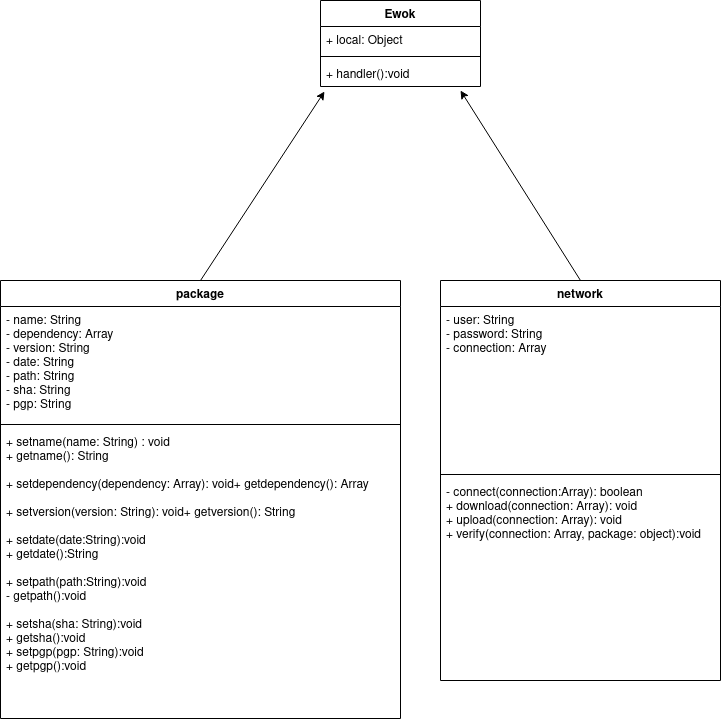
\includegraphics[width=0.8\linewidth,clip=]{./img/Klassendiagramm.png}%
\captionof{figure}{Klassendiagramm}%
\label{fig:Klassendiagramm}%
\end{minipage}
\vspace{10px}





\section{Use-Case-Diagramm}
\begin{minipage}{\linewidth}
\centering%
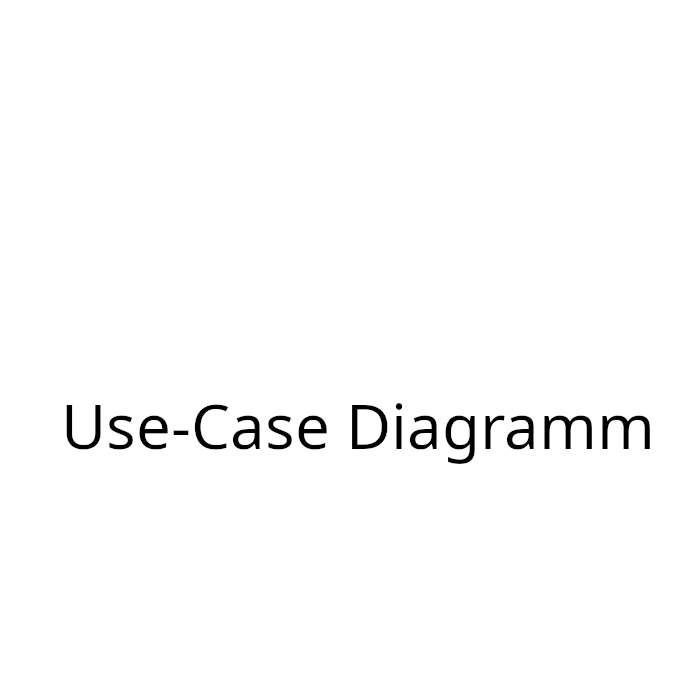
\includegraphics[width=0.8\linewidth,clip=]{./img/Use-Case-Diagramm.png}%
\centering
\captionof{figure}{Use-Case-Diagramm}%
\label{fig:Use-Case-Diagramm}%
\end{minipage}
\vspace{10px}


%% Syntax
% This file is a ghost. Only abbreviations for foreign words or new words are stored here. Nothing more

\nomenclature{RION}{Package-Manager und Schnittstelle für die Packetverwaltung zwischen X-FAB-Server und Client}

\nomenclature{X-FAB}{X-FAB ist ein Anbieter für Halbleitertechnologien, welche die Fertigung als auch Desiginunterstützung für Kunden anbietet, die gemischt analog-digitale integrierte Schaltkreise (ICs) entwickeln. \cite{XFAB}}

\nomenclature{INOR}{Serverseitiges BackEnd bei X-FAB}

\nomenclature{Pakete / Packages}{Datenbündel, die als solches eine Funktion haben. (Hiermit sind die Pakete auf den X-FAB Servern gemeint)}

\nomenclature{paru}{Ein AUR-Helper, der es erlaubt unter Arch-Linux und darauf basierenden Distributionen Pakete aus der AUR zu installieren, aktualiesieren, etc.}

\nomenclature{Python}{Programmiersprache: \url{https://www.python.org/}}

\nomenclature{CLI}{Ein \texttt{C}ommand \texttt{L}ine \texttt{I}nterface ist eine Schnittstelle, die es dem Nutzer erlaubt, Textbefehle an ein Programm zu übermitteln. Betriebssysteme, darunter GNU/Linux stellen hierfür eine sogennate Shell, wie zum Beispiel Bash, Dash oder ZSH, zur Verfügung, auf welche man mit einem Terminal zugreifen kann.}

\nomenclature{Manpage}{Eine Hilfeseite für installierte Programme unter Unix-artigen Systemen, auf der, für gewöhnlich, Befehle, Flags und Hinweise zur Benutzung eines Programms verzeichnet sind. Darauf zugriffen wird mit \texttt{man >>name<<} aufrufen.}

\nomenclature{PyPi}{Pypi ist ein Software Sammlung wo Python Packages via pip heruntergeladen werden können}

\nomenclature{pip}{Python Package Manager: \url{https://pypi.org/project/pip/}}


%%% Ende %%%

\appendix
\part*{Anhang}


% Anahng
%% ++++++++++++++++++++++++++++++++++++++++++++++++++++++++++++
%% Anhang: Literaturverzeichnis
%% ++++++++++++++++++++++++++++++++++++++++++++++++++++++++++++


% Mit dem Befehl \nocite werden auch nicht im Text zitierte
% aus der Literaturdatenbank mit in das Literaturverzeichnis aufgenommen.
% Ein "\nocite{*}" übernimmt ungeprüft die komplette Datenbank.
%\nocite{*}

\cleardoublepage
\nocite{*}
\ihead[]{Literaturverzeichnis}
\bibliographystyle{acm}
\bibliography{literatur} % "literatur.bib" ist hier die einzige Literaturdatenbank.

% Alternativ: Mehrere Datenbanken verwenden, falls eine
% oder mehrere umfangreiche Sammlungen exisitieren:
%\bibliography{literatur_buecher,literatur_weblinks}


%% ++++++++++++++++++++++++++++++++++++++++++++++++++++++++++++
%% Anhang: Abbildungsverzeichnis
%% ++++++++++++++++++++++++++++++++++++++++++++++++++++++++++++


% Keine Änderungen vornehmen!
\cleardoublepage
\ihead[]{Abbildungsverzeichnis}
\listoffigures


%% ++++++++++++++++++++++++++++++++++++++++++++++++++++++++++++
%% Anhang: Abkürzungsverzeichnis
%% ++++++++++++++++++++++++++++++++++++++++++++++++++++++++++++


% Hier keine weiteren Änderungen vornehmen
\cleardoublepage
\ihead[]{Abkürzungsverzeichnis und Formelzeichen}
\printnomenclature{} % TODO: Hyperref




\end{document}
